\chapter{Densidades}\label{cap:densidades}

\begin{proposicion}[{\guia{Teorema 10.1}, \cite[Prop.~2.1.1]{nualart2006}}]
Si $F\in\Dom$ y $\D F/\norm{\D F}_\Hil^2\in\operatorname{Dom}\dive$, $F$ tiene densidad
continua
\[
  p_F(x)=\E\Big[\ind_{\{F>x\}}\,\dive\Big(\frac{\D F}{\norm{\D F}^2_\Hil}\Big)\Big].
\]
\end{proposicion}

Para $F=S_T$: $\D F=\sigma S_T\ind_{[0,T]}$, $\norm{\D F}^2=\sigma^2S_T^2T$ y
\[
  \dive\Big(\frac{1}{\sigma TS_T}\Big)=\frac1{S_T}\Big(\frac{W_T}{\sigma T}+1\Big).
\]
El estimador resultante es insesgado en cada punto y no requiere ancho de banda.
Las mismas ideas sustentan la expansión de la volatilidad implícita en
\cite{alos2007,alosgarcialorite2021}.

\begin{figure}[h]
  \centering
  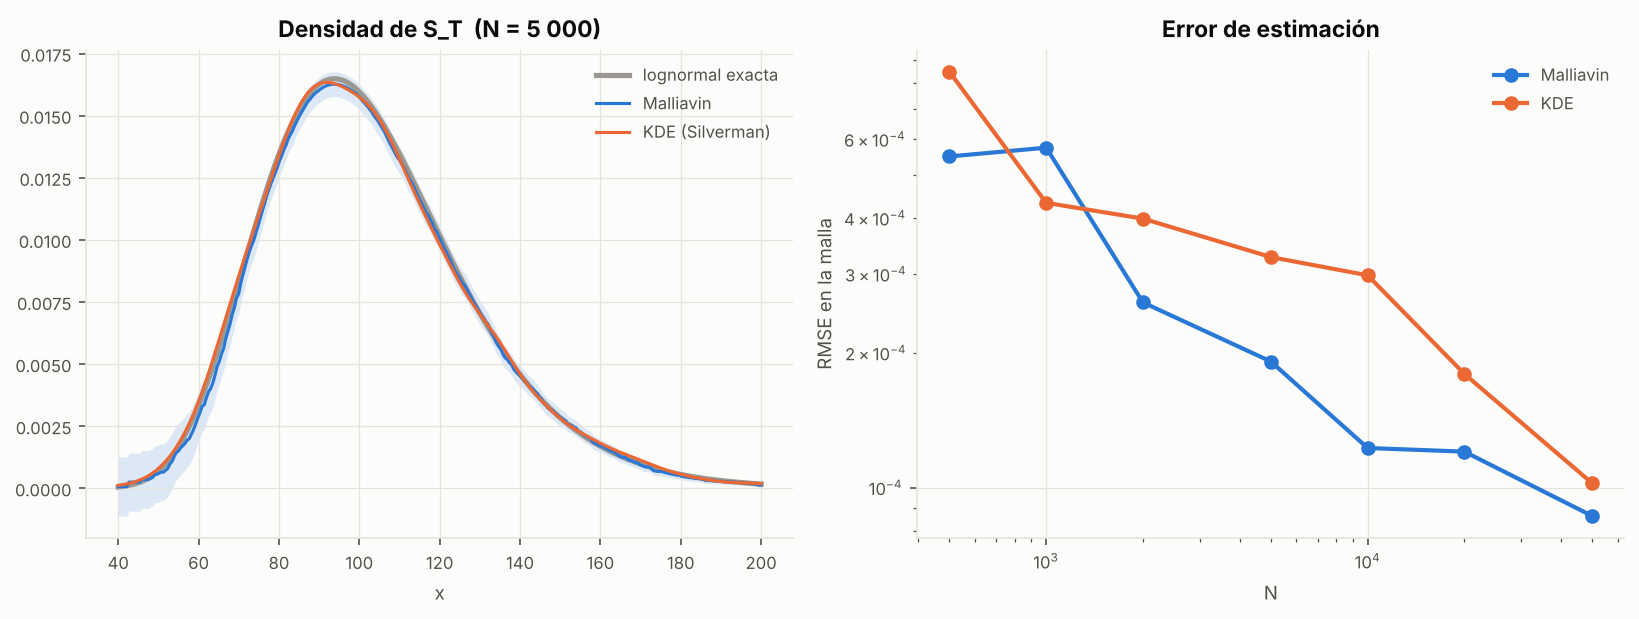
\includegraphics[width=0.95\linewidth]{06_densidad_malliavin}
  \caption{Densidad de $S_T$: Malliavin vs.\ KDE (\codigo{examples/06\_densidad\_malliavin.py}).}
\end{figure}
